\documentclass{article}
    \usepackage[ukrainian]{babel} 
    \newtheorem{theorem}{Теорема}
    \usepackage{amssymb}
    \usepackage{amsmath}
    \usepackage[14pt]{extsizes}
    \textheight=24cm
    \textwidth=16cm
    \oddsidemargin=0pt
    \topmargin=-1.5cm
    \def\baselinestretch{1.5}
    \usepackage{amsfonts}
    \usepackage{graphicx}
    \usepackage{color}
    \usepackage{alltt}
    \parindent=1cm
    \usepackage{indentfirst}
    \graphicspath{{pictures/}}
    
\begin{document}
Титульный лист
\pagebreak
\tableofcontents
\pagebreak

%==================ВСТУП===================================================================%
\section{Вступ}

Стабілізація нелінійних систем є однією з найбільш цікавих та важливих задач теорії керування.
Не дивлячись на великі досягнення останніх десятеліть %Korobov, Halil% 
ця задача досі не розв'язана в 
загальному випадку. Особливий інтерес викликають системи нестабілізовані за першим
наближенням~\cite{BebiyaKorobov}, \cite{Bebiya}.

Один з найбільш універсальних методів стабілізації нелінійних систем є метод зворотнього ходу 
(backstepping в англомовній літературі).% Helicopters, Halil%
 Метод зворотнього ходу - це рекурсивна процедура, в котрій поєднані задачі пошуку функції Ляпунова та відповідного закону
керування. Суть методу полягає у тому, що задача пошуку закону керування всієї системи розбиваеться на послідовність
відповідних підзадач для підсистем меншого порядку, для яких уже відомий закон керування та функція Ляпунова.
Зі зростанням розмірності кожна додаткова фазова змінна входить як керування у нову підсистему. 
При такому підході суттєвим є вимога трикутності системи.

Клас трикутних систем було введено В.І.~Коробовим у роботі~\cite{Korobov} при розляді задачі
керування супутником.
Трикутною системоа має вигляд: 
\begin{equation}\label{M1}
	\begin{cases}
        \dot x_1 = f_1(x_1, x_2)\\
        \dot x_2 = f_2(x_1, x_2 ,x_3)\\
        \cdot \quad \cdot \quad \cdot \quad \cdot \quad \cdot \quad \cdot \quad\\
        \dot x_{n-1} = f_{n-1}(x_1, \dots ,x_n)\\
        \dot x_{n} = f_{n}(x_1, \dots ,x_n,u)\\
	\end{cases}
\end{equation}

У роботі~\cite{Korobov} була доведена достатня умова повної керованості та стабілізованості
системи~(\ref{M1}). А саме було доведено, що для повної керованості та стабілізованості
системи~(\ref{M1}) достатньо, щоб при деякому $a>0$ виконувалась наступна
умова 
\begin{equation}\label{M2}
    \frac{\partial f_i(x_1,\dots,x_{i+1})}{\partial x_{i+1}} \geq a > 0 
\end{equation} 
для всіх $x_1, \dots, x_{i+1}$, $i=1 \dots n $ ($x_{n+1} = u$). При цьому 
припускалося, що виконані такі умови на гладкість правої частини: 
$ f_i(x_1,\dots,x_{i+1})$ $\in$ $\mathbb{C}^{n-i}$, $i=1 \dots n $ ($x_{n+1} = u$).

У данній дипломній роботі розглядається випадок трикутних систем спеціального вигляду при відсутності вищезначених вимог
щодо гладкості правої  частини системи~(\ref{M1}). 
Також ці системи не задовільняють умові~(\ref{M2}), тому в роботі було адаптовано метод 
зворотньго ходу для дослідження таких систем.  Використовуючи цей підхід вдалося 
побудовати функцію Ляпунова та стабілізуюче керування. 
\pagebreak

%==================ЗАГАЛЬНИЙ ВИГЛЯД====================================================================%
\section{Метод зворотнього ходу для трикутних систем}
\subsection{Загальний вигляд трикутної системи для застосування методу зворотнього ходу}
У даному розділі буде стисло описана сутність методу зворотньго ходу та умови  
при виконанні яких є можливим застосування данного методу до трикутних систем. Більш детально 
робота методу буде продемонстрована у розділі 2.2 на прикладі двовимірної системи.

Для того, щоб застосовувати метод зворотньго ходу система повинна мати наступний вигляд:
\begin{equation} \label{strict-feedback system}
    \begin{cases}
        \dot x           = f_0(x)+g_0(x)\xi_1\\
        \dot \xi_1       = f_1(x, \xi_1)+g_{1}(x, x_1)\xi_2 \\
        \dot \xi_2       = f_2(x, \xi_1, \xi_2) + g_2(x, \xi_1, \xi_2)\xi_3 \\
       \cdot \quad \cdot \quad \cdot \quad \cdot  \quad \cdot  \quad \cdot
        \quad \cdot  \quad \cdot  \quad \cdot  \quad \cdot  \quad \cdot\\

       \dot \xi_{n-1}   = f_{n-1}(x, \xi_1, \xi_2, ... ,\xi_{n-1}) 
        +g_{n-1}(x, \xi_1, \xi_2, ... ,\xi_{n-1}) \xi_n\\
        \dot \xi_{n}     = f_{n}(x, \xi_1, \xi_2, ... ,\xi_{n}) 
        +g_{n}(x, \xi_1, \xi_2, ... ,\xi_{n})u\\

	\end{cases}
\end{equation}


Де $x \in \mathbb{R}$, $n \leq 1$\\
$\xi_1, \xi_2, ... ,\xi_n \in \mathbb{R}$, $u \in \mathbb{R}$ - керування,\\ 
$f_i, g_i, i = 1 ... n $ -  відомі функції, $f_i(0,0, \dots, 0) = 0$, 
$g_i(x,z_1, \dots, z_n) \neq 0$
Такі трикутні системи ще називають "strict-feedback" системи.\\
Розглянемо наступну підсистему в системі ~(\ref{strict-feedback system}):

\begin{equation} \label{strict-feedback small subsystem}
\dot x = f_0(x)+g_0(x)u_1
\end{equation}

Важливо, щоб система ~(\ref{strict-feedback small subsystem}) була стабілізована будь-яким іншим способом.
Припускаємо,що для системи~(\ref{strict-feedback small subsystem}) 
відомі функція Ляпунова та стабілізуюче керування.
Далі за допомогою методу зворотнього ходу можемо "приєднувати" рівняння к початковій системі, 
збільшучи на кожному кроці розмірниість системи на один. 

Знаючи стабілізуюче керування для підсистеми  ~(\ref{strict-feedback small subsystem})
можемо стабілізувати систему ~(\ref{2dim strict-feedback system}) наступним чином:
\begin{equation} \label{2dim strict-feedback system}
    \begin{cases}
    \dot x = f_0(x)+g_0(x)\xi_1\\
    \dot \xi_1 = f_1(x,\xi_1)+g_1(x,\xi_1)u_1(x,\xi_1)\\
    \end{cases}
\end{equation}

Знаходимо керування $u_1(x,\xi_1)$ таке, щоб підсистема
\begin{equation}
    \dot \xi_1 = f_1(x,\xi_1)+g_1(x,\xi_1)u_1(x,\xi_1)
\end{equation}
була стабілізована. Знаходження стабілізуючого керування базується на побудові наступної функції Ляпунова:

\begin{equation}
V_{1}(x,\xi_1)=V_{1}(x)+{\frac{1}{2}}(\xi_1-u_{0}(x))^{2}
\end{equation}
Вибераємо $u_1(x,\xi_1)$ так, щоб $\dot V_{1} < 0$.
Таким чином, система ~(\ref{2dim strict-feedback system}) стабілізована.
 
Аналогічно, будуємо керування $u_{2}(x,\xi_{1},\xi_{2})$
для підсистеми 
\begin{equation*}
    \dot \xi_2 = f_1(x,\xi_1,\xi_2)+g_1(x, \xi_1, \xi_2)u_2(x,\xi_1, \xi_2)
\end{equation*} 

Функція Ляпунова:
\begin{equation*}
    V_{2}(x,\xi_{1}, \xi_{2})=V_{1}(x,\xi_{1})+{\frac {1}{2}}(\xi_{2}-u_{1}(x,\xi_{1}))^{2}
\end{equation*}
Вибераємо $u_2(x,\xi_1, \xi_2)$ так, щоб $\dot V_{2} \le 0$

Можемо повторити процедуру $n$ разів поки не знайдемо керування $u$ для всієї системи~(\ref{strict-feedback system})

%========================================================================================================%
\pagebreak



%==================Стабілізація двовим системи===============================================================================%
\subsection{Стабілізація двовимірної системи за допомогою методу зворотнього ходу}
Розглянемо систему:
\begin{equation}
	\begin{cases}
		\dot \xi_1 = f(\xi_1) + g(\xi_1)\xi_2 \\
		\dot\xi_2 = u
	\end{cases}
\end{equation}

Ця система може бути розглянута як дві підсистеми, а саме перша підсистема, де $\xi_2$ виступає як вхід, друга
підсистема, як інтегратор. Основна ідея побудови полягае у тому, щоб розгядати $\xi_2$ як (віртуальне) керування для
стабілізації $\xi_1$. Вважаемо, що існує керування $\phi(\xi_1)$, таке, що нульова точка покою
системи $\dot \xi_1 = f(\xi_1) + g(\xi_1)\phi(\xi_1)$
асимптотично стійка.
Вважаемо, що для вибраного $\phi(\xi_1)$ функція Ляпунова $V(\xi_1)$  відома та задовільняє умові:

\begin{equation}
    \frac{\partial V(\xi)}{\partial \xi_1}(f(\xi_1)+g(\xi_1)\phi(\xi_1)) \leq
    -W(\xi_1), \forall \xi_1 \in \mathbb{R}
\end{equation}
До першого рівняння додамо та віднімемо $g(\xi_1)\phi(\xi_1)$

\begin{eqnarray}
\dot\xi_1 &=& f(\xi_1)+g(\xi_1)\phi(\xi_1)-g(\xi_1)\phi(\xi_1)+g(\xi)\xi_2\\
&=&f(\xi_1)+g(\xi_1)\phi(\xi_1)-g(\xi_1)(\phi(\xi_1)-\xi_2)
\end{eqnarray}
Позначимо $e_{\xi_1} = \xi_2-\phi(\xi_1)$
Перепишемо систему в координатах $(\xi_1, e_{\xi_1})$

\begin{equation}
    \begin{cases}
    \dot \xi_1 = (f(\xi_1)+g(\xi_1)\phi(\xi_1))+g(\xi_1)e_{\xi_1}\\
    \dot e_{\xi_1} = u-\dot \phi(xi_1)\\  
    \end{cases}
\end{equation}
Обчислити $\dot\phi$ 

\begin{equation}
    \dot\phi = \frac{\partial \phi}{\partial \xi_1}(f(\xi_1)+g(\xi_1)\xi_2)
\end{equation}
Позначимо: $u = v + \dot\phi$, $v \in \mathbb{R}$.
Систему перепишемо:
\begin{equation}
    \begin{cases}
        \dot \xi_1 = (f(\xi_1)+g(\xi_1)\phi(\xi_1))+g(\xi_1)e_{\xi_1}\\
        \dot e_{\xi_1} = v\\
    \end{cases}
\end{equation}
Відмітемо, що система має асимтотично стійку нульову точку спокою $\xi_1$ коли $e_{\xi_1}$
Розглянемо функцію $V(\xi_1,\xi_2)$ - кандидат на функцію Ляпунова, що має вигляд:
\begin{eqnarray}
    \dot V_2 &=& \frac{\partial V}{\partial \xi_1}(f(\xi_1)+g(\xi_1)\phi(\xi_1))+
    \frac{\partial V}{\partial \xi_1}e_{\xi_1}+e_{\xi_1}v\\
    &\leq& -W(\xi_1)+ \frac{\partial V}{\partial \xi_1}e_{\xi_1}+e_{\xi_1}v
\end{eqnarray}

У якості $\dot e_{\xi_1}$ беремо 
\begin{equation}
    v = - \frac{\partial V}{\partial \xi_1}g(\xi_1) - ke_{\xi_1}
\end{equation}

Параметр $k$ вибераємо додатним.
Отримаємо $V_2 \leq -W(\xi_1) - ke_{(\xi_1)^2}$ \\
Таким чином $\phi(0)=0$, $e_{\xi_1} -> 0$ нульова точка покою асимптотично стійка.
Кінцевий вигляд закону керування:

\begin{equation}
    u = \frac{\partial \phi}{\partial \xi_1}(f(\xi_1)+g(\xi_1)\xi_2)-
    \frac{\partial V}{\partial \xi_1}g(\xi_1)-k(\xi_2-\phi(\xi_1))
\end{equation}

Аналогічним способом:
\begin{equation} \label{2dim system last step}
    \begin{cases}
        \dot \xi_1 = f_1(\xi_1)+g_1(\xi_1)(\xi_2 + \phi_1(\xi_1)-\phi_1(\xi_1))\\
        \dot \xi_2 = u = f_2(\xi_1,\xi_2)+g(\xi_1,\xi_2)\xi_3\\
    \end{cases}
\end{equation}
~(\ref{2dim system last step})

\begin{equation}
    \xi_3 = \frac{u - f_2(\xi_1, \xi_2)}{g_2(\xi_1, \xi_2)} = \phi(\xi_1,\xi_2)
\end{equation}

Повертаючись до задачі стабілізації вихідної системи~(\ref{strict-feedback system}) 
повторюємо процедуру $n$ разів, після чого отримаємо наступну послідовність функцій $\phi_i$:

$\phi_1(\xi_1)$, $\phi_2(\xi_1,\xi_2)$, $\phi_2(\xi_1,\xi_2,\xi_3)$, $\dots$,
$\phi_{n-1}(\xi_1,\xi_2, \dots, \xi_{n-1})$\\
та функцію Ляпунова:
\begin{equation}
    V_n = V(x)+\frac{1}{2}(\xi_2-\phi_1(\xi_1))^2 + \dots 
    +\frac{1}{2}(\xi_2-\phi_{n-1}(\xi_1, \dots, \xi_{n-1}))^2
\end{equation}

%==========================================================================================================%
\pagebreak
\section{Стабілізація системи с двома степеневими нелінійностями}
\subsection{Постановка задачі стабілізації системи с двома степеневими нелінійностями}
У даній роботі розглядається наступна трикутна система
\begin{equation}\label{nonlinear system with ^3}
    \begin{cases}
    \dot x_1 = x_2^3 \\
    \dot x_2 = \xi_1^3\\
    \dot \xi_1 = f(x_1, x_2,\xi_1) + g(x_1, x_2, \xi_1)\xi_2 \\
    \cdot \quad \cdot \quad \cdot \quad \cdot  \quad \cdot  \quad \cdot
    \quad \cdot  \quad \cdot  \quad \cdot  \quad \cdot  \quad \cdot\\
    \dot \xi_n = f(x_1, x_2,\xi_1,\xi_2, \dots, \xi_n) + 
    g(x_1, x_2, \xi_1,\xi_2, \dots, \xi_n)u \\
    \end{cases}
\end{equation}

Метою даної роботи є стабілізація системи ~(\ref{nonlinear system with ^3}), тобто пошук такого
керування u, що нульова точка спокою системи буде асимтотично стійкою. 

Для вирішення данної задачі
використовуємо метод зворотнього ходу, що був описаний у розділі 2. Звернемо увагу, на відміну від 
системи ~(\ref{strict-feedback system}) фазова змінна $\xi_1$ входить у наступне рівняння нелінійно,
а саме як третя ступінь $\xi_1^3$
\pagebreak


%=======================SECTION_4=========================================================================%
\subsection{Розв'язок задачі стабілізації системи с двома степеневими нелінійностями}
Розглянемо наступну систему:
\begin{equation}\label{3dim nonlinear system}
    \begin{cases}
    \dot x_1 = x_2^3 \\
    \dot x_2 = \xi_1^3\\
    \dot \xi_1 = u\\
    \end{cases}
\end{equation}

Для стабілізації системи~(\ref{Mar12}) потрібно спочатку знайти функцію Ляпунова
та керування для підсистеми, що на розмірність менше ніж система  тобто розглянемо 
наступну підсистему другого порядку. 
\begin{equation} \label{2dim nonlinear system}
    \begin{cases}
    \dot x_1 = x_2^3\\
    \dot x_2 = v^3\\
    \end{cases}
\end{equation}
До першого рівняння додамо та віднімемо вираз $(ax_1+bx_2)^3$:
\begin{equation}\label{m15}
    \begin{cases}
    \dot x_1 = x_{2}^3 \\
    \dot x_2 = v^3 - (ax_1+bx_2)^3 +(ax_1+bx_2)^3 \\
    \end{cases}
\end{equation}
В якості допоміжного керування $v$ візмемо $v=ax_1+bx_2$, $a,b \in \mathbb{R}$. Тоді
для стабілізації підсистеми~(\ref{m15}) потрібно занйти такі  $a,b$ щоб нульова точка спокою 
наступної системи
\begin{equation}\label{2dim nonlinear system2}
    \begin{cases}
    \dot x_1 =x_{2}^3 \\
    \dot x_2 =(ax_1+bx_2)^3 \\
    \end{cases}
\end{equation}
була асимтотичног стійкою.


До правої частини першого рівняння додамо та віднімемо функцію $\gamma^3(x_1)$ 
\begin{equation} \label{m17}
    \begin{cases}
    \dot x_1 =x_{2}^3 -\gamma^3(x_1)+\gamma^3(x_1) \\
    \dot x_2 = (ax_1+bx_2)^3,\\
    \end{cases}
\end{equation}
де $\gamma(x_1) = \alpha x_1$.

Функцію Ляпунова візьмемо у вигляді  
\begin{equation}
    V = \frac{1}{2}x_{1}^2 +\frac{1}{2}c(x_2 - \gamma(x_1) )^2\\
\end{equation}

Знайдемо похідну функціїї Ляпунова в силу системи~(\ref{m17}):
\begin{eqnarray}
    \dot V =&& x_1 \Big (x_2^3 - \gamma^3(x_1)+\gamma^3(x_1) \Big) +\nonumber \\
    &&c(x_2 - \gamma(x_1)
    \Big((ax_1+bx_2)^3-\frac{\partial \gamma(x_1)}{\partial x_1}x_2^3 \Big)
\end{eqnarray}

Після перетворень маємо:
\begin{eqnarray}
    \dot V&=& x_1\gamma^3(x_1)+c(x_2 - \gamma(x_1))
   \Big (x_1x_2^2 + x_1x_2\gamma(x_1) + x_{1}\gamma^2(x_1) +\nonumber\\ 
    &&(ax_1+bx_2)^3 - \frac{\partial \gamma(x_1)}{\partial x_1}x_{2}^3\Big)
\end{eqnarray}

Для того, щоб похідна функції Ляпунова $\dot V$ була від'ємною, представимо
 $\dot V$ як квадратичну форму, що має вигляд $\dot V =(Gy,y)$ 
та вибрати матрицю $G$ таку, щоб  $\dot V =(Gy,y) < 0$.

Знайдемо $a,b$ щоб при деяких $p, \beta$ виконувалась наступна рівність:
\begin{eqnarray}
    x_1x_2^2+x_1x_2\gamma(x_1) + x_1 \gamma^2(x_1) - 
    c\frac{\partial \gamma(x_1)}{\partial x_1}x_2^3 + c(ax_1+bx_2)^3 = \nonumber\\
    -p(x_2-\gamma(x_1))^3 +2\beta(x_2-\gamma(x_1))x_{1}^2 
\end{eqnarray}

Оскільки $\gamma(x_1)=\alpha x_1$, де $\alpha \in \mathbb{R}$,
отримаємо наступне рівняння:
\begin{eqnarray}
x_1x_{2}^2 + \alpha x_{1}^2x_2 &+& \alpha^2x_{1}^3 -c\alpha x_{2}^3 
+ ca^3x_{1}^3 +c b^3x_{2}^3 + c3ba^2x_{1}^2x_2+\nonumber
c3ab^2x_1x_{2}^2 =\\
-p(x_2^3 - \alpha^{3}x_{1}^3 &-& 3\alpha x_2^2x_{1} + 3\alpha^2x_2x_{1}^2)+
2\beta x_2x_{1}^2 - 2\alpha \beta x_1^3
\end{eqnarray}

Для знаходження параметрів отримаємо наступну систему алгебраїчних рівнянь 
\begin{equation}
    \begin{cases}
        -c\alpha+cb^3+p=0\\
        \alpha^2+ca^3-p\alpha^3+2\alpha\beta=0\\
        \alpha+c3ba^2+3p\alpha^2-2\beta=0\\
        1+c3ab^2-3\alpha p=0\\
    \end{cases}
\end{equation}

Розв'язуючи  систему отримали такі значення параметрів $a$, $b$, $\beta$, $p$: 
\begin{equation}
    \begin{cases}
        b = -\frac{1}{3}\sqrt{3}
            (z)^{\frac{1}{6}}\\
        a=  \frac{1}{3}\sqrt{3}\frac{ \sqrt{z} \alpha c+9\alpha^2 c-3}
        {z^{\frac{1}{3}}c}\\
        p= \frac{1}{9}c(\sqrt{3}\sqrt{z}+9\alpha)\\
        \beta = -\frac{1}{2} 
        \frac{9\sqrt{3}\alpha^4c^2+3\sqrt{z}\alpha^3c^2
        -6\sqrt{3}\alpha^{2}c - 3\sqrt{z}\alpha c +\sqrt{3}
        }{c\sqrt{z}}
    \end{cases}
\end{equation}

Де $z = \frac{(3\alpha^2c-1)^3}{\alpha^2c^2(\alpha^2c-3)}$.

Таким чином можемо представити $\dot V$ як квадратичну форму:
\begin{eqnarray}\label{nonlinear dV}
    \dot V &=& \alpha^3x_{1}^4 - p(x_2-\gamma(x_1))^4
    +2\beta(x_2-\gamma(x_1))^2x_{1}^2\nonumber\\ 
    &=&\alpha^3x_{1}^4 + 2\beta(x_2-\alpha x_1)^2x_{1}^2
    -p(x_2-\alpha x_1)^4
\end{eqnarray}

Відмітемо що рівність ~(\ref{nonlinear dV}) можно представити у вигляді $\dot V =(Gy,y)$, де 
мариця $G$ та вектор $y$ мають вигляд: 
\begin{equation}
G=\left(\begin{array}{clr}
    \alpha^3 & \beta\\
    \beta & -p
\end{array}\right) 
\end{equation}

\begin{equation}
    y=(x_{1}^2,(x_2-\alpha x_{1})^2)
\end{equation}

Матриця G є від'ємно визначена при виконнані наступних умов:

1) $\alpha^3 < 0$, ~$p > 0$

2) Детермінант матриці $G$ додатній, тобто $\beta^2<-\alpha^3p$


Таким чином при виконнані вищезазначених умов 
керування $ v=(ax_1+bx_2)$ стабілізує підсистему~(\ref{2dim nonlinear system}).

Для того щоб переконатись, що умови () можуть бути виконані розглянемо наступний 
приклад. 

{\bfПриклад~1}.

Покладемо значення параметрів $\alpha$, $c$ як: $\alpha = -2$, $c = 1$
тоді матриця $G$ буде дорівнювати:
\begin{equation}
    G=\left(\begin{array}{clr}
        -8 & 3.255437356\\
        3.255437356 & -1.510566062
    \end{array}\right) 
    \end{equation}

Обчисливши визначник матриці $G$ переконалися, що він додатній та дорівнює $det(G)=1.48665612$.

Стабілізуюче керування для вихідної системи~(\ref{2dim nonlinear system})
дорівнює:

$u = (-1.519820798x_1(t)-1.452240544x_2(t))^3$

Побудуємо графіки траєкторій:
\begin{figure}[h]
    \center{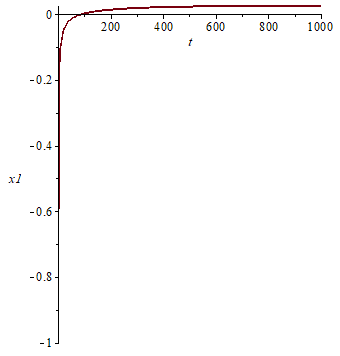
\includegraphics[scale=0.5]{trject1}}
    \caption{traject1}
    \label{fig:image1}
\end{figure}

\begin{figure}[]
    \center{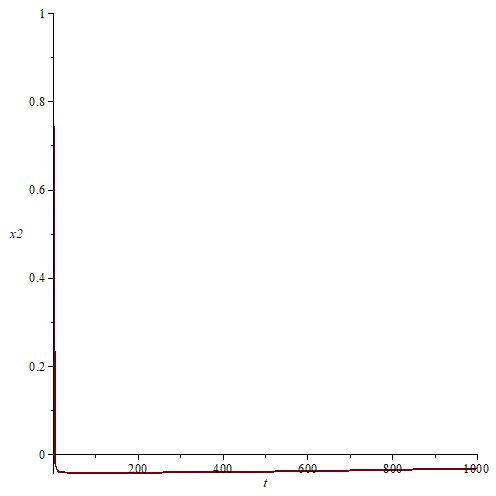
\includegraphics[scale=0.5]{trject2}}
    \caption{traject2}
    \label{fig:image2}
\end{figure}

\begin{figure}[]
    \center{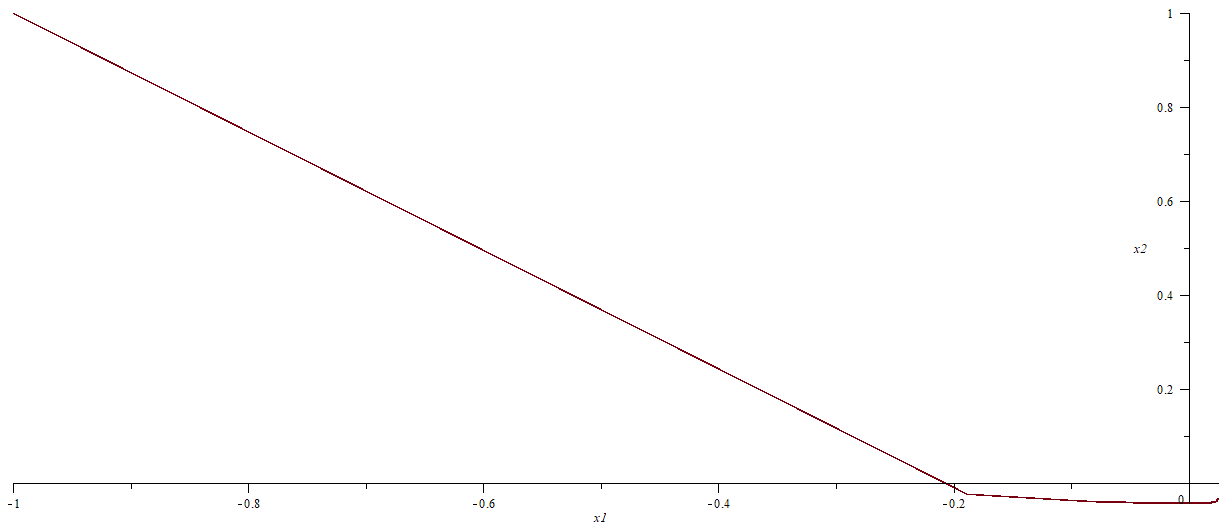
\includegraphics[scale=0.3]{trject3}}
    \caption{traject3}
    \label{fig:image3}
\end{figure}

\pagebreak

Використовуючи метод зворотнього ходу від підсистеми ~(\ref{2dim nonlinear system}) 
перейдемо до системи   ~(\ref{3dim nonlinear system}), де  в якості $u$ візьмемо:

$f_1(x_1,x_2,\xi_1)+g_2(x_1,x_2,\xi_1)\xi_2$.

\begin{equation} \label{3dim nonlinear system step2}
    \begin{cases}
        \dot x_1 = x_2^3 \\
        \dot x_2 = \xi_1^3\\
        \dot \xi_1 =f_1(x_1,x_2,\xi_1)+g_1(x_1,x_2,\xi_1)\xi_2 = v_1\\
        \end{cases}
\end{equation}

Із системи ~(\ref{3dim nonlinear system step2}) отримаємо керування $\xi_2$ 
\begin{equation}
    \xi_2 = \frac{v_1-f_1(x_1,x_2xi_1)}{g_1(x_1,x_2,\xi_{1})}, ~g \neq 0
\end{equation}

Запишемо функцію Ляпунова:
\begin{equation}
    V_1 = V+\frac{1}{2}(\xi_1-v)^2=\frac{1}{2}x_1^2+\frac{1}{2}(x_2-\gamma(x_1))^2+
    \frac{1}{2}(\xi_1-v)^2
\end{equation}

Де $v = ax_1+bx_2$ та $\gamma(x_1) = \alpha x_1$

Обчислимо похідну функції Ляпунова $V_1$:
\begin{eqnarray}
    \dot V_1 &=& \dot V + (x_2-\alpha x_1) \Big( \xi_1-(ax_1+bx_2) \Big)
    \Big( \xi_1^2+\xi_1+(ax_1+bx_2) \nonumber \\ &+&(ax_1+bx_2)^2 \Big)
    +(\xi_1+(ax_1+bx_2))
    \Big(u-\frac{\partial v}{\partial x_1}x_{2}^3 
    - \frac{\partial v}{\partial x_2}\xi_{1}^3 \Big)
\end{eqnarray}

Використовуючи вже доведене раніше твердженя, що похідна функції Ляпунова $\dot V$ для системи
 ~(\ref{2dim nonlinear system2})  меньше ніж нуль, потрібно вибрати таке $v_1$, що для похідної функції
Ляпунова $\dot V_1$ буде також виконуватися умова $\dot V_1 < 0$.

$v_1$ виберемо наступним чином:
\begin{eqnarray}
    v_1 &=& \frac{\partial v}{\partial x_1}x_{2}^3 + \frac{\partial v}{\partial x_2}\xi_{1}^3
    - (x_2 -\alpha x_1) \Big(\xi_1^2 + \xi_1(ax_1 + bx_2) \nonumber \\ 
    &+& (ax_1+bx_2)^2 \Big) -(\xi_1 - ax_1-bx_2)
\end{eqnarray}
Тоді отримаємо
\begin{equation}
    \dot V_1 = \dot V - (\xi_1 - v)^2<0
\end{equation}

Таким чином похідна функії Ляпунова $ \dot V_1 <0$, тобто нульова точка покою системи асимтотично 
стійка. Можемо зробити висновок, що система з керуванням стабілізована.
Застосовуючи метод зворотньго ходу до системи ~(\ref{3dim nonlinear system step2}) можемо послідовно під'єднувати
рівняння, збільшуючи на кожному кроці розмірність системи на один. 
\begin{equation}
{\begin{cases}
{\begin{cases}
{\begin{cases}
{\begin{cases}
{\begin{cases}
{\begin{cases}
{\begin{cases}
{\begin{cases}
\dot x_1 = x_2^3 \\
\dot x_2 = \xi_1^3\\
{\dot  {\xi}}_{1}=f_{1}(x,\xi_{1})+g_{1}(x,\xi_{1})\xi_{2}\end{cases}}\\
{\dot  {\xi}}_{2}=f_{2}(x,\xi_{1},\xi_{2})+g_{2}(x,\xi_{1},\xi_{2})\xi_{3}\end{cases}}\\\vdots \\\end{cases}}\\
{\dot  {\xi}}_{i}=f_{i}(x,\xi_{1},\xi_{2},\ldots ,\xi_{i})+g_{i}(x,\xi_{1},\xi_{2},\ldots ,\xi_{i})\xi_{{i+1}}\end{cases}}\\\vdots \end{cases}}\\
{\dot  {\xi}}_{{k-2}}=f_{{k-2}}(x,\xi_{1},\xi_{2},\ldots \xi_{{k-2}})+g_{{k-2}}(x,\xi_{1},\xi_{2},\ldots ,\xi_{{k-2}})\xi_{{k-1}}\end{cases}}\\
{\dot  {\xi}}_{{k-1}}=f_{{k-1}}(x,\xi_{1},\xi_{2},\ldots \xi_{{k-2}},\xi_{{k-1}})+g_{{k-1}}(x,\xi_{1},\xi_{2},\ldots ,\xi_{{k-2}},\xi_{{k-1}})\xi_{k}\end{cases}}\\
{\dot  {\xi}}_{k}=f_{k}(x,\xi_{1},\xi_{2},\ldots \xi_{{k-1}},\xi_{k})+g_{k}(x,\xi_{1},\xi_{2},\ldots ,\xi_{{k-1}},\xi_{k})u\\\end{cases}}
\end{equation}
Де починаючи $i=2$ керування $u$ в загальному випадку має вид:

\begin{eqnarray}
u_{i} =\frac{1}{g_{i}(x_1, x_2, \xi_1, \xi_2, \dots ,\xi_i)}
    (v_{i-1}-f_{i}(x_1, x_2, \xi_1, \xi_2, \dots ,\xi_i))
\end{eqnarray}
де $v_i$:

\begin{eqnarray}
    v_{i}=
\end{eqnarray}


\pagebreak
\section{Висновки}
В данній роботі дослідженно питання стабілізованості для  трикутної симтеми спеціального 
вигляду, що не може бути відобажена на лінійну систему існуючими методами. Зокрема 
для цієї системи невиконана відома умова  відображуваності В. І. Коробова.

У першому розділі було описано загальний метод зворотньго 
ходу для трикутних систем лінійних за однією з координат,
що мають вигляд ().

У другому розділі запропоновано рекурсивну процедуру побудави функції Ляпунова та стабілізуючого керування 
для системи. 
Розглянуто випадок у якому невиконується умова лінійності за відповідною
координатою, а саме було розглянуто трикутну систему з двома однаковими ступеневими нелінійностями. 
Для випадку зростання ступенів дана задача була вирішена в роботі().  
Спочатку була розв'язана задача стабілізація для двовимірної канонічної симтеми 
з двома ступеневими нелінійностями. Використовуючи метод зворотного ходу був здійснений перехід від стабілізації двовимірної системи
до стабілізації багатовимірної системи. Отримані результати проілюстровані відповідними прикладами.











%В даній роботі була розглянута стабілізація нелінійних систем, зокрема трикутних систем зі ступеневою нелінійністю.
%В. І. Коробовим були отримані достатні умови при яких трикутна система відображається на лінійну канонічну 
%систему та є повністю керованою та стабілізованою. В роботі розглядалася система для якої ці
%достатні умови невиконані тому така система не може бути відображена на лінійну. Тому для таких систем
%було застосовано метод зворотньго ходу. 

%У данній роботі вдалося модифікувати метод зворотного ходу для застосування до 
%трикутних систем зі ступеневою нелінійністю більш високого порядку. 
%Складність у тому, що раніше метод зворотного ходу застосовувався до систем лінійних за однією з координат.
%Спочатку, розвинувши результати Бебії М. О., в роботі була розв'язана  задача стабілізації 
%для системи з двома степеневими нелінійностями. 
%Використовуючи рекурсивну процедуру методу зворотного ходу  був здійснен переход  від 
%стабілізації  тривимірної системи  до стабілізації n-вимірної системи. 



\pagebreak
\begin{thebibliography}{}
    \bibitem{Korobov} 
    В.~И.~Коробов, Управляемость, устойчивость некоторых нелинейных систем, 
    -  Дифференц. уравнения, 1973, том 9, номер 4, с. 614-619.\\
    \bibitem{BebiyaKorobov} 
    M.~O.~Bebiya, V.~I.~Korobov, On stabilization problem for nonlinear system power principal part. 
    - Joyrnal of Mathematical Physics, Analysis, Geometry 2016, Vol. 12, No. 2, pp. 113-133.\\
    \bibitem{backstepping}
    I.A. Raptis, K.P. Valavanis, Linear and Nonlinear Control of Small-Scale Unmanned Helicopters, 
    Intelligent Systems, Control and Automation: Science and Engineering 45, 
    DOI 10.1007/978-94-007-0023-9, © Springer Science+Business Media B.V. 2011\\
    \bibitem{Bebiya}  
    М.~О.~Бебия, "Стабилизация систем со степенной нелинейностью". Вісник ХНУ ім. В.~Н.~Каразіна. 
    Серія "Математика, прикладна математика і механіка" №1120, 2014. сс.75-84.\\
\end{thebibliography}

\end{document}